\subsection{IFIT2AB Discussion}\label{subsec:IFIT2AB Discussion}
\subsubsection{Discussion About Differences Seen Between the Two Antibodies in Previous Subchapter} \label{Disuccion sadf}
IFIT2A shows monkey IFIT2 forming inclusion within the pIB structure, while also colocalising with the pIB-associated filamentous network.  IFIT2B shows exclusion from both pIB and the filaments.

IFIT2A shows overexpressed hIFIT2-FLAG to form inclusion inside the pIBs and colocalization with the filamentous network. IFIT2B also shows inclusion inside the pIBs but shows potential exclusion from the filamentous network.
IFIT2A shows colocalization to the ring and inner edge of human IBs with occasional inclusions. IFIT2B shows complete and partial exclusion from the human IB structures. 

IFT2A shows bovine IFIT2 col9ocalisation to the with the ring structure of bovine IBs. IFIT2B shows partial exclusion; exclusion from the IB ring and inner edge with IBAG-like inclusions; and diffusion through the IB structure.
\subsubsection{Differences Between the Two Antibodies Other Than IB Staining} \label{Differences Between the Two Antibodies Other Than IB Staining}
\myparagraph{Human Protein Atlas Show Cytoplasmic Localisation Similar to IFIT2B} \label{Human Protein Atlas Show Cytoplasmic Localisation Similar to IFIT2B}

\begin{figure}
    \centering
    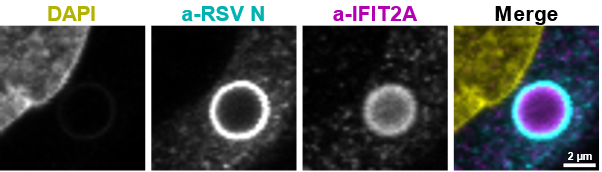
\includegraphics[width=1\linewidth]{10. Chapter 5//Figs//01. I2A/04. i2a a549 hrsv n.png}
    \caption[example ifi2a hrsv]{example ifi2a hrsv}
    \label{fig:example ifi2a hrsv}
\end{figure}

IFIT2A antibody shows mainly cytoplasmic distribution (although some spots are visible)


\begin{figure}
    \centering
    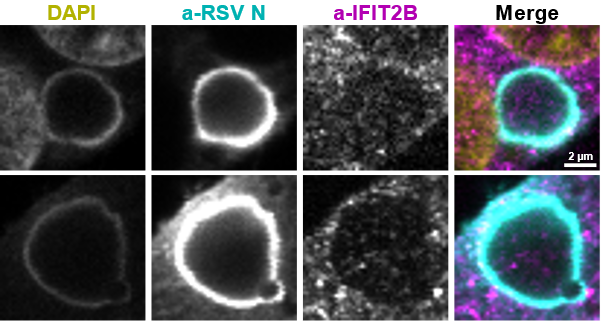
\includegraphics[width=1\linewidth]{10. Chapter 5//Figs//02. I2B/03. i2b a549 hrsv n.png}
    \caption[example ifi2b hrsv]{example ifi2b hrsv}
    \label{fig:example ifi2b hrsv}
\end{figure}

IFIT2B shows mainly granular/vesicular distribution.

\begin{figure}
    \centering
    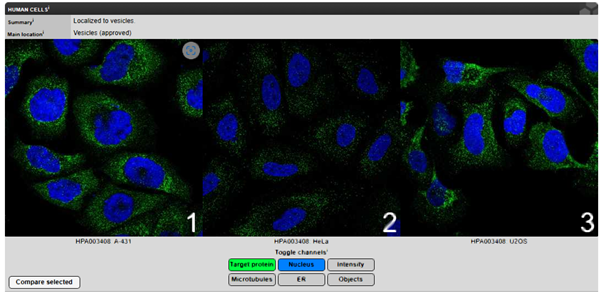
\includegraphics[width=1\linewidth]{10. Chapter 5//Figs//04. IFIT2AB Discussion/02. human protein atlas ifit2.png}
    \caption[human protein atlas ifit2]{human protein atlas ifit2}
    \label{fig:human protein atlas ifit2}
\end{figure}

Human protein atlas shows vesicular distribution of IFIT2.
Side note: second figure from section 1.1.1.2.3 shows cytoplasmic staining (like IFIT2A, but kinetochore microtubule staining (like IFIT2B).

\myparagraph{P Transfection Induces IFIT2A Signal but not IFIT2B Signal} \label{P Transfection Induces IFIT2A Signal but not IFIT2B Signal}
Cell Line: 293T \newline
Treatment: hN and/or hP (EV – empty vector) \newline
Detecting magenta: endogenous human IFIT2 (A) \newline
Detecting cyan: N and/or P \newline

IFIT2 induction detected in hP and hP + hN conditions, suggesting that transfection of P induces IFIT2 expression (but this does not happen with IFIT1 or IFIT3 in the same cells).
About the different genomic regulation landscape… why does IFIT2 get induced but not other IFITs (within human genome which is well annotated)? 
Side note: No kinetochore microtubule staining (especially in first panel)

\begin{figure}
    \centering
    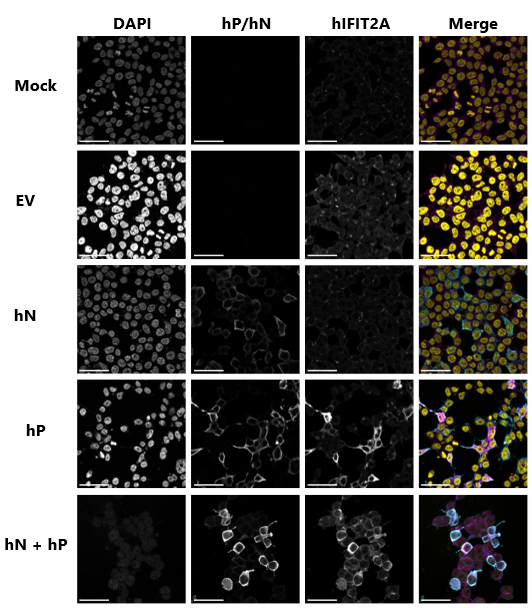
\includegraphics[width=1\linewidth]{10. Chapter 5//Figs//04. IFIT2AB Discussion/03. ifit2a p transfection.png}
    \caption[ifit2a p transfection]{ifit2a p transfection}
    \label{fig:ifit2a p transfection}
\end{figure}

Cell Line: 293T \newline
Treatment: hN and/or hP (EV – empty vector) \newline
Detecting magenta: endogenous human IFIT2 (B) \newline
Detecting cyan: N and/or P \newline

No detected IFIT2 induction in any of the conditions.
Side note: We can see kinetochore microtubule staining, especially in the first row.

\begin{figure}
    \centering
    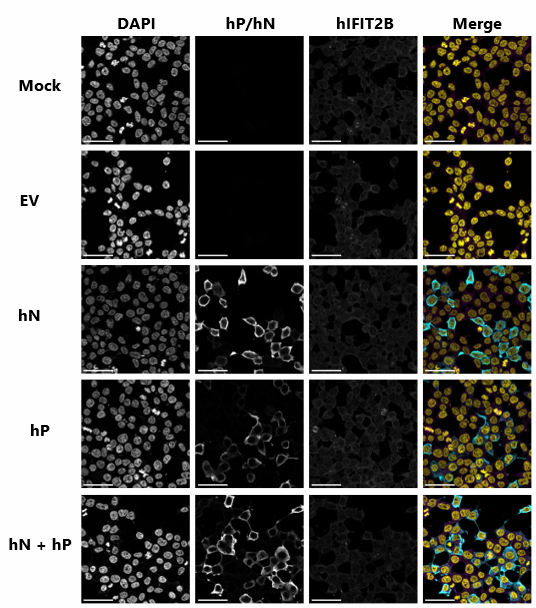
\includegraphics[width=1\linewidth]{10. Chapter 5//Figs//04. IFIT2AB Discussion/04. ifit2b p transfection.png}
    \caption[ifit2b p transfection]{ifit2b p transfection}
    \label{fig:ifit2b p transfection}
\end{figure}

\myparagraph{IFIT2B but not IFIT2A Stains Kinetochore Microtubules} \label{IFIT2B but not IFIT2A Stains Kinetochore Microtubules}
Cell Line: MDBK \newline
Treatment: bRSV + bIFNa \newline
Detecting magenta: endogenous human IFIT2 (B) \newline
Detecting cyan: bovine IBs \newline

IFIT2B antibody consistently stains kinetochore microtubules in all cells regardless of the condition. This was figure that I had done already which had the kinetochore microtubule staining present, hence I included it here. I found only one minor paper about IFIT2 localisation that shows the same staining. Literature search looking at kinetochore proteomes never mentioned IFIT2, neither papers about anaphase/metaphase proteome.

\begin{figure}
    \centering
    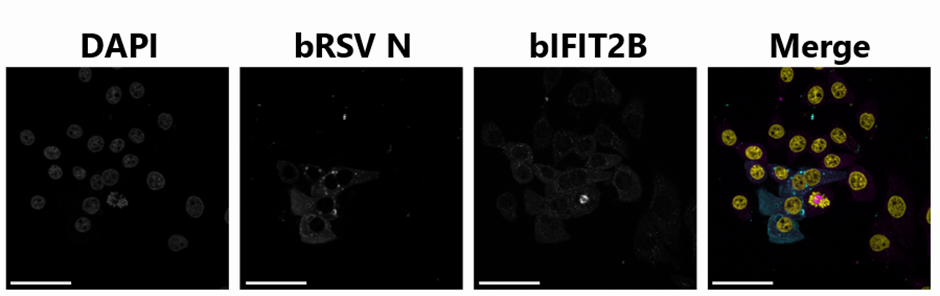
\includegraphics[width=1\linewidth]{10. Chapter 5//Figs//04. IFIT2AB Discussion/05. kinetochores.png}
    \caption[kinetochores]{kinetochores}
    \label{fig:kinetochores}
\end{figure}

This is figure from the paper that mentions mouse IFIT2 (GARG39) to be associated with microtubules during the different phases of cell cycle.
Side note: The IFIT2 distribution is cytoplasmic and not vesicular, like human protein atlas suggests.

\begin{figure}
    \centering
    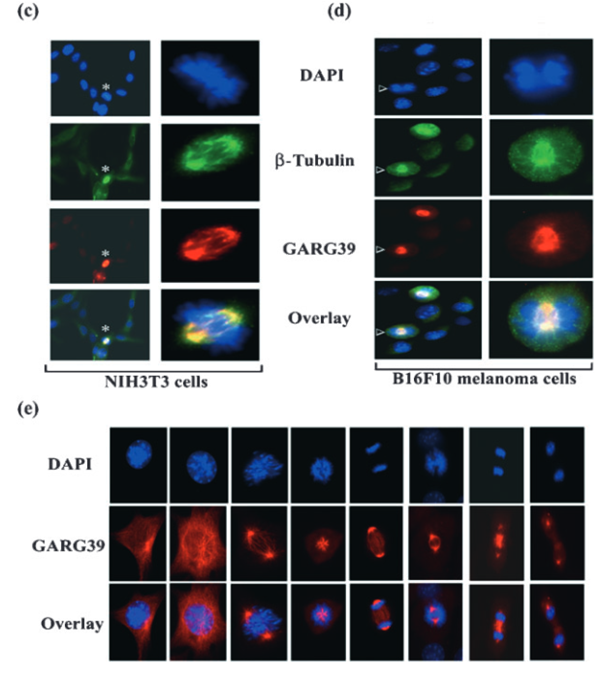
\includegraphics[width=1\linewidth]{10. Chapter 5//Figs//04. IFIT2AB Discussion/06. kinetochore published figure.png}
    \caption[kinetochore published figure]{kinetochore published figure}
    \label{fig:kinetochore published figure}
\end{figure}

\myparagraph{WB antibody validation} \label{WB antibody validation}
Western blots below are a validation of IFIT antibodies cross-reactivity. They are 293T cells transfected with empty vector or highlighted IFITs.

We see less material to be present in bovine samples, especially bovine IFIT3 sample.

IFIT2A antibody detects overexpressed human and bovine IFIT2, while also detecting overexpressed human and bovine IFIT3. We see differential staining between IFIT2A and IFIT3 antibody, hence we can conclude that IFIT2A is not detecting IFIT3 in IF analyses. IFIT2A is also detecting a moiety at 25 kDa, which we do not know the origin of (cellular sources as it is present in empty vector as well).

IFIT2B antibody detects human IFIT2. It fails to detect bovine IFIT2, however, this could be due to lower reactivity with the bovine IFIT2 and/or lower expression levels in that sample. Unlike in IFIT2A antibody, we see no reactivity with IFIT3. As with IFIT2A antibody, we are detecting 25 kDa moiety in all conditions.

\begin{figure}
    \centering
    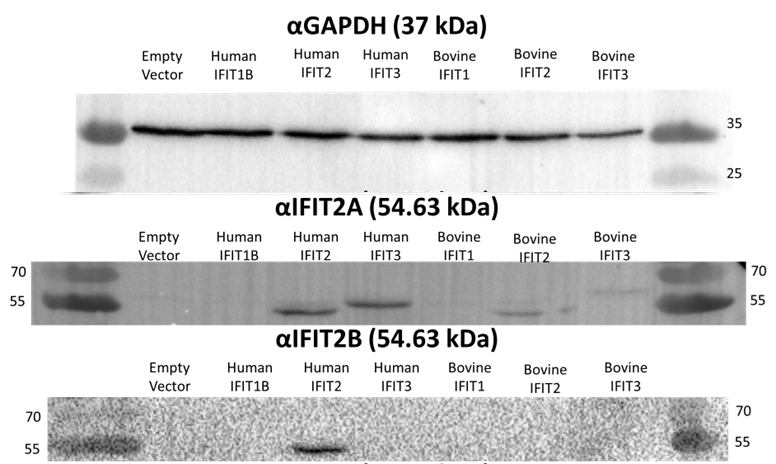
\includegraphics[width=1\linewidth]{10. Chapter 5//Figs//04. IFIT2AB Discussion/07. antibodies ifit2.png}
    \caption[ifit2 antibodies figure]{ifit2 antibodies figure}
    \label{fig:ifit2 antibodies figure}
\end{figure}

\subsubsection{Summary} \label{Summary-ab discussion}
We were thinking that the differential staining between IFIT2A and IFIT2B antibodies could be due epitope masking (due to e.g. RNA interaction; interaction with other IFITs; interaction with other cellular proteins; interaction with viral proteins) but although both of the antibodies seem to detect IFIT2 in western bots, they differ quite substantially in other aspects. One fails to capture induction caused by P transfection, while the other fails to capture kinetochore microtubule staining.